\section{Evietania Charis Sujadi(1174051)}
\subsection{Intalasi Map Proxy}
\begin{enumerate}
    \item Gunakan perintah pip install map proxy pada cmd
    \hfill\break
    \begin{figure}[H]
		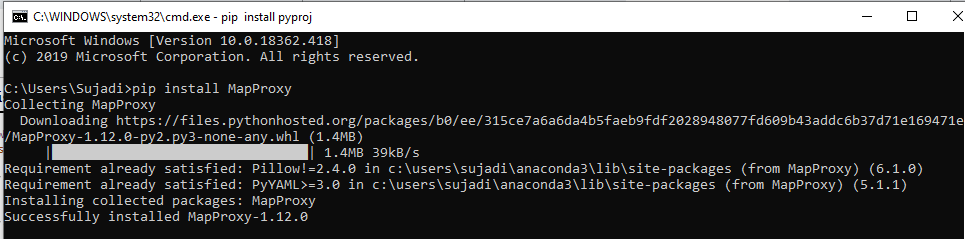
\includegraphics[width=4cm]{figures/1174051/5/4.png}
		\centering
		\caption{Perintah untuk menginstal map proxy}
    \end{figure}
    \item Gunakan perintah pip install pyproj
    \hfill\break
    \begin{figure}[H]
		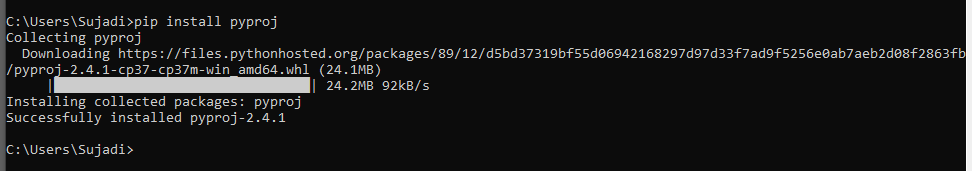
\includegraphics[width=4cm]{figures/1174051/5/14.png}
		\centering
		\caption{Perintah untuk mengantisipasi jika terjadi error}
    \end{figure}
\end{enumerate}
\subsection{Konfigurasi}
\begin{enumerate}
    \item Buka file agm.yaml
    \hfill\break
    \begin{figure}[H]
		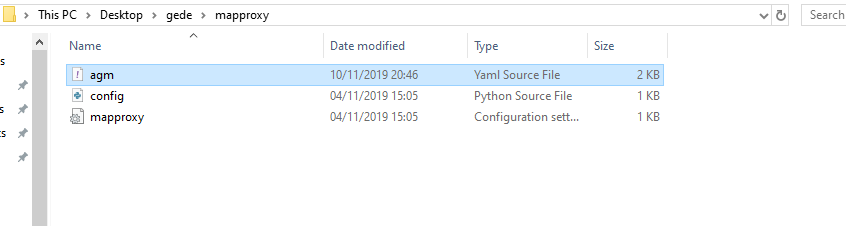
\includegraphics[width=4cm]{figures/1174051/5/15.png}
		\centering
		\caption{Buka filenya}
    \end{figure}
    \item Buka file agm.yaml, dan edit
    \hfill\break
    \begin{figure}[H]
		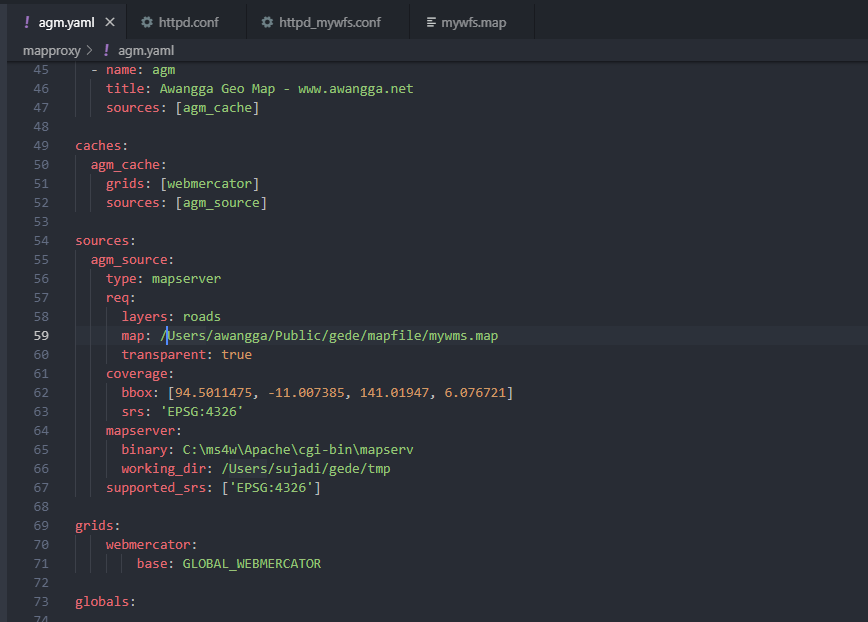
\includegraphics[width=4cm]{figures/1174051/5/16.png}
		\centering
		\caption{Buka filenya dan edit}
    \end{figure}
    untuk binarynya sesuai dengan tempat map servernya
\end{enumerate}
\subsection{Pengujian}
\begin{enumerate}
    \item Untuk melakukan pengujian bisa dengan menggunakan perintah mapproxy-util serve-develop mapproxy.yaml -b 0.0.0.0:8181
    \hfill\break
    \begin{figure}[H]
		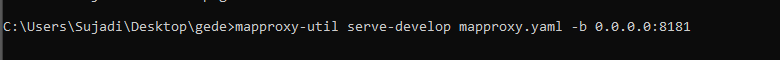
\includegraphics[width=4cm]{figures/1174051/5/17.png}
		\centering
		\caption{Perintah untuk menjalankan mapproxy}
    \end{figure}
\end{enumerate}
\subsection{Link Youtube}
\href{https://www.youtube.com/watch?v=pC5HCwQ0atE&feature=youtu.be}{Klik Disini}